% !TEX program = xelateDtx
\documentclass[a4paper,11pt]{ctexart}

\ProvidesFile{mathnote-preamble.tex}[2024/11/13 Math note modern preamble]
\RequirePackage{iftex}
\ifPDFTeX
  \PackageError{mathnote-preamble}{请使用 \XeLaTeX\ 或 LuaLaTeX 编译该模板}{在 MikTeX / TeX Live 中切换到 \XeLaTeX\ (推荐) 或 LuaLaTeX 后重新编译。}
\fi
\makeatletter
\newif\ifmathnote@fontdirfound
\mathnote@fontdirfoundfalse
\def\mathnote@fontdircandidates{fonts/,./fonts/,../fonts/,../../fonts/,../../../fonts/}
\def\mathnote@fontdir{}
\@for\mathnote@cand:=\mathnote@fontdircandidates\do{%
  \ifmathnote@fontdirfound\else
    \IfFileExists{\mathnote@cand NotoSerif-VF.ttf}{%
      \edef\mathnote@fontdir{\mathnote@cand}%
      \mathnote@fontdirfoundtrue
    }{%
      \IfFileExists{\mathnote@cand SourceHanSerifSC-Regular.otf}{%
        \edef\mathnote@fontdir{\mathnote@cand}%
        \mathnote@fontdirfoundtrue
      }{}%
    }%
  \fi
}
\ifmathnote@fontdirfound\else
  \edef\mathnote@fontdir{fonts/}%
\fi
\@ifundefined{MathNoteFontDir}{%
  \edef\MathNoteFontDir{\mathnote@fontdir}%
}{}

% --------------------------------------------------
% User switches
% --------------------------------------------------
\newif\ifmathnoteprintmode
\mathnoteprintmodefalse
\newcommand{\MathNoteEnablePrint}{%
  \mathnoteprintmodetrue
  \mathnote@applypalette
}
\newif\ifmathnotereviewstamp
\mathnotereviewstampfalse
\newcommand{\mathnote@reviewstamppathbase}{assest/lzlxV-reviewed}
\newcommand{\mathnote@reviewstampsvg}{\mathnote@reviewstamppathbase.svg}
\newcommand{\mathnote@reviewstamppdf}{\mathnote@reviewstamppathbase.pdf}
\newcommand{\mathnote@reviewstampinclude}{}
\newif\ifmathnote@reviewstampplaced
\mathnote@reviewstampplacedfalse
\IfFileExists{\mathnote@reviewstamppdf}{%
  \renewcommand{\mathnote@reviewstampinclude}{%
    \includegraphics[width=20mm,height=20mm,keepaspectratio]{\mathnote@reviewstamppdf}%
  }%
}{%
  \IfFileExists{\mathnote@reviewstampsvg}{%
    \renewcommand{\mathnote@reviewstampinclude}{%
      \includesvg[width=20mm,height=20mm,keepaspectratio]{\mathnote@reviewstamppathbase}%
    }%
  }{}%
}
\newcommand{\mathnote@enablereviewstamp}{%
  \ifx\mathnote@reviewstampinclude\@empty
    \PackageWarning{mathnote-preamble}{Review stamp graphic \mathnote@reviewstampsvg\space (or PDF fallback) not found}%
  \else
    \mathnote@reviewstampplacedfalse
    \AddToHook{shipout/foreground}{%
      \ifmathnote@reviewstampplaced\else
        \begin{tikzpicture}[remember picture, overlay]
          \node[anchor=north east, xshift=-8mm, yshift=-8mm] at (current page.north east){%
            \mathnote@reviewstampinclude
          };
        \end{tikzpicture}%
        \global\mathnote@reviewstampplacedtrue
      \fi
    }%
  \fi
}
\newcommand{\MathNoteEnableReviewStamp}{%
  \mathnotereviewstamptrue
  \mathnote@enablereviewstamp
}

% --------------------------------------------------
% Metadata defaults (can be overwritten in each file)
% --------------------------------------------------
\providecommand{\notetitle}{数学学习笔记}
\providecommand{\noteauthor}{作者}
\providecommand{\notedate}{\today}
\providecommand{\notesubtitle}{现代数学排版示例}
\providecommand{\noteversion}{v1.0}

% --------------------------------------------------
% Core packages
% --------------------------------------------------
\usepackage{geometry}
\geometry{
  paper=a4paper,
  top=2.35cm,
  bottom=2.4cm,
  left=2.1cm,
  right=2.1cm,
  headheight=16pt,
  headsep=14pt
}

\usepackage{fontspec}
\usepackage{metalogo}
\defaultfontfeatures{Ligatures=TeX, Scale=MatchLowercase}

\newcommand{\mathnote@fontfile}[1]{\MathNoteFontDir#1}
\newif\ifmathnote@haslocalserif
\newif\ifmathnote@haslocalsans
\newif\ifmathnote@haslocalmono
\newif\ifmathnote@haslocalcjkserif
\newif\ifmathnote@haslocalcjksans
\newif\ifmathnote@haslocalcjkmono
\newif\ifmathnote@haslocalkai
\newif\ifmathnote@haslocalshserif
\newif\ifmathnote@haslocalshsans
\IfFileExists{\mathnote@fontfile{NotoSerif-VF.ttf}}{\mathnote@haslocalseriftrue}{\mathnote@haslocalseriffalse}
\IfFileExists{\mathnote@fontfile{NotoSans-VF.ttf}}{\mathnote@haslocalsanstrue}{\mathnote@haslocalsansfalse}
\IfFileExists{\mathnote@fontfile{NotoSansMono-VF.ttf}}{\mathnote@haslocalmonotrue}{\mathnote@haslocalmonofalse}
\IfFileExists{\mathnote@fontfile{NotoSerifCJK-VF.ttc}}{\mathnote@haslocalcjkseriftrue}{\mathnote@haslocalcjkseriffalse}
\IfFileExists{\mathnote@fontfile{NotoSansCJK-VF.ttc}}{\mathnote@haslocalcjksanstrue}{\mathnote@haslocalcjksansfalse}
\IfFileExists{\mathnote@fontfile{NotoSansMonoCJK-VF.ttc}}{\mathnote@haslocalcjkmonotrue}{\mathnote@haslocalcjkmonofalse}
\IfFileExists{\mathnote@fontfile{LXGWWenKaiSC-Regular.ttf}}{\mathnote@haslocalkaitrue}{\mathnote@haslocalkaifalse}
\IfFileExists{\mathnote@fontfile{SourceHanSerifSC-Regular.otf}}{\mathnote@haslocalshseriftrue}{\mathnote@haslocalshseriffalse}
\IfFileExists{\mathnote@fontfile{SourceHanSansSC-Regular.otf}}{\mathnote@haslocalshsanstrue}{\mathnote@haslocalshsansfalse}

\newcommand{\mathnote@cjkitalicfont}{}
\newcommand{\mathnote@cjkitalicfeatures}{Language = Chinese Simplified}
\ifmathnote@haslocalkai
  \def\mathnote@cjkitalicfont{LXGWWenKaiSC-Regular}
  \def\mathnote@cjkitalicfeatures{Path = {\MathNoteFontDir}, Extension = .ttf, Language = Chinese Simplified}
\else
  \IfFontExistsTF{LXGW WenKai SC}{%
    \def\mathnote@cjkitalicfont{LXGW WenKai SC}%
    \def\mathnote@cjkitalicfeatures{Language = Chinese Simplified}
  }{%
    \def\mathnote@cjkitalicfont{}%
    \def\mathnote@cjkitalicfeatures{Language = Chinese Simplified}
  }%
\fi
\ifx\mathnote@cjkitalicfont\@empty
  \def\mathnote@cjkitalicfont{FandolKai}
  \def\mathnote@cjkitalicfeatures{Language = Chinese Simplified}
\fi

\newcommand{\mathnote@setlatinfonts}{%
  \ifmathnote@haslocalserif
    \setmainfont{Noto Serif}[
      Path = {\MathNoteFontDir},
      Extension = .ttf,
      UprightFont = NotoSerif-VF,
      ItalicFont = NotoSerif-Italic-VF,
      BoldFont = NotoSerif-VF,
      BoldFeatures = {RawFeature={+wght=760}},
      BoldItalicFont = NotoSerif-Italic-VF,
      BoldItalicFeatures = {RawFeature={+wght=760}}
    ]%
  \else
    \IfFontExistsTF{Noto Serif}{%
      \setmainfont{Noto Serif}[
        ItalicFont = {Noto Serif Italic},
        BoldFont = {Noto Serif Bold},
        BoldItalicFont = {Noto Serif Bold Italic}
      ]%
    }{%
      \setmainfont{TeX Gyre Pagella}%
    }%
  \fi
  \ifmathnote@haslocalsans
    \setsansfont{Noto Sans}[
      Path = {\MathNoteFontDir},
      Extension = .ttf,
      UprightFont = NotoSans-VF,
      ItalicFont = NotoSans-Italic-VF,
      BoldFont = NotoSans-VF,
      BoldFeatures = {RawFeature={+wght=760}},
      BoldItalicFont = NotoSans-Italic-VF,
      BoldItalicFeatures = {RawFeature={+wght=760}}
    ]%
  \else
    \IfFontExistsTF{Noto Sans}{%
      \setsansfont{Noto Sans}[
        ItalicFont = {Noto Sans Italic},
        BoldFont = {Noto Sans Bold},
        BoldItalicFont = {Noto Sans Bold Italic}
      ]%
    }{%
      \setsansfont{TeX Gyre Heros}%
    }%
  \fi
  \ifmathnote@haslocalmono
    \setmonofont{Noto Sans Mono}[
      Path = {\MathNoteFontDir},
      Extension = .ttf,
      UprightFont = NotoSansMono-VF,
      BoldFont = NotoSansMono-VF,
      BoldFeatures = {RawFeature={+wght=740}},
      ItalicFont = NotoSansMono-VF,
      ItalicFeatures = {FakeSlant=0.2}
    ]%
  \else
    \IfFontExistsTF{Noto Sans Mono}{%
      \setmonofont{Noto Sans Mono}[
        BoldFont = {Noto Sans Mono Bold}
      ]%
    }{%
      \setmonofont{TeX Gyre Cursor}%
    }%
  \fi
}

\newcommand{\mathnote@setcjkfonts}{%
  \ifmathnote@haslocalshserif
    \setCJKmainfont{SourceHanSerifSC-Regular}[
      Path = {\MathNoteFontDir},
      Extension = .otf,
      Language = Chinese Simplified,
      BoldFont = SourceHanSerifSC-Bold,
      ItalicFont = {\mathnote@cjkitalicfont},
      ItalicFeatures = {\mathnote@cjkitalicfeatures}
    ]%
  \else
    \IfFontExistsTF{Source Han Serif SC}{%
      \setCJKmainfont{Source Han Serif SC}[Language=Chinese Simplified, ItalicFont={\mathnote@cjkitalicfont}, ItalicFeatures={\mathnote@cjkitalicfeatures}]%
    }{%
      \ifmathnote@haslocalcjkserif
        \setCJKmainfont{NotoSerifCJK-VF}[
          Path = {\MathNoteFontDir},
          Extension = .ttc,
          Language = Chinese Simplified,
          UprightFont = NotoSerifCJK-VF,
          UprightFeatures = {FontIndex=2},
          BoldFont = NotoSerifCJK-VF,
          BoldFeatures = {FontIndex=2,RawFeature={+wght=780}},
          AutoFakeSlant = 0.18,
          ItalicFont = {\mathnote@cjkitalicfont},
          ItalicFeatures = {\mathnote@cjkitalicfeatures}
        ]%
      \else
        \IfFontExistsTF{Noto Serif CJK SC}{%
          \setCJKmainfont{Noto Serif CJK SC}[Language=Chinese Simplified, ItalicFont={\mathnote@cjkitalicfont}, ItalicFeatures={\mathnote@cjkitalicfeatures}]
        }{%
          \setCJKmainfont{FandolSong}[BoldFont={FandolSong-Bold}, ItalicFont={\mathnote@cjkitalicfont}, ItalicFeatures={\mathnote@cjkitalicfeatures}]
        }%
      \fi
    }%
  \fi
  \ifmathnote@haslocalshsans
    \setCJKsansfont{SourceHanSansSC-Regular}[
      Path = {\MathNoteFontDir},
      Extension = .otf,
      Language = Chinese Simplified,
      BoldFont = SourceHanSansSC-Bold,
      ItalicFont = {\mathnote@cjkitalicfont},
      ItalicFeatures = {\mathnote@cjkitalicfeatures}
    ]%
    \setCJKfamilyfont{hei}{SourceHanSansSC-Regular}[
      Path = {\MathNoteFontDir},
      Extension = .otf,
      BoldFont = SourceHanSansSC-Bold
    ]%
  \else
    \IfFontExistsTF{Source Han Sans SC}{%
      \setCJKsansfont{Source Han Sans SC}[Language=Chinese Simplified, ItalicFont={\mathnote@cjkitalicfont}, ItalicFeatures={\mathnote@cjkitalicfeatures}]
      \setCJKfamilyfont{hei}{Source Han Sans SC}[Language=Chinese Simplified]
    }{%
      \ifmathnote@haslocalcjksans
        \setCJKsansfont{NotoSansCJK-VF}[
          Path = {\MathNoteFontDir},
          Extension = .ttc,
          Language = Chinese Simplified,
          UprightFont = NotoSansCJK-VF,
          UprightFeatures = {FontIndex=2},
          BoldFont = NotoSansCJK-VF,
          BoldFeatures = {FontIndex=2,RawFeature={+wght=780}},
          ItalicFont = {\mathnote@cjkitalicfont},
          ItalicFeatures = {\mathnote@cjkitalicfeatures}
        ]%
        \setCJKfamilyfont{hei}{NotoSansCJK-VF}[
          Path = {\MathNoteFontDir},
          Extension = .ttc,
          UprightFont = NotoSansCJK-VF,
          UprightFeatures = {FontIndex=2},
          BoldFont = NotoSansCJK-VF,
          BoldFeatures = {FontIndex=2,RawFeature={+wght=820}}
        ]%
      \else
        \IfFontExistsTF{Noto Sans CJK SC}{%
          \setCJKsansfont{Noto Sans CJK SC}[Language=Chinese Simplified, ItalicFont={\mathnote@cjkitalicfont}, ItalicFeatures={\mathnote@cjkitalicfeatures}]
          \setCJKfamilyfont{hei}{Noto Sans CJK SC}[Language=Chinese Simplified]
        }{%
          \setCJKsansfont{FandolHei}[ItalicFont={\mathnote@cjkitalicfont}, ItalicFeatures={\mathnote@cjkitalicfeatures}]
          \setCJKfamilyfont{hei}{FandolHei}
        }%
      \fi
    }%
  \fi
  \ifmathnote@haslocalshsans
    \setCJKmonofont{SourceHanSansSC-Regular}[
      Path = {\MathNoteFontDir},
      Extension = .otf,
      Language = Chinese Simplified,
      BoldFont = SourceHanSansSC-Bold,
      ItalicFont = {\mathnote@cjkitalicfont},
      ItalicFeatures = {\mathnote@cjkitalicfeatures}
    ]%
  \else
    \IfFontExistsTF{Source Han Sans SC}{%
      \setCJKmonofont{Source Han Sans SC}[Language=Chinese Simplified, ItalicFont={\mathnote@cjkitalicfont}, ItalicFeatures={\mathnote@cjkitalicfeatures}]
    }{%
      \ifmathnote@haslocalcjkmono
        \setCJKmonofont{NotoSansMonoCJK-VF}[
          Path = {\MathNoteFontDir},
          Extension = .ttc,
          Language = Chinese Simplified,
          UprightFont = NotoSansMonoCJK-VF,
          UprightFeatures = {FontIndex=2},
          BoldFont = NotoSansMonoCJK-VF,
          BoldFeatures = {FontIndex=2,RawFeature={+wght=760}},
          ItalicFont = {\mathnote@cjkitalicfont},
          ItalicFeatures = {\mathnote@cjkitalicfeatures}
        ]%
      \else
        \IfFontExistsTF{Noto Sans Mono CJK SC}{%
          \setCJKmonofont{Noto Sans Mono CJK SC}[Language=Chinese Simplified, ItalicFont={\mathnote@cjkitalicfont}, ItalicFeatures={\mathnote@cjkitalicfeatures}]
        }{%
          \setCJKmonofont{FandolFang}[ItalicFont={\mathnote@cjkitalicfont}, ItalicFeatures={\mathnote@cjkitalicfeatures}]
        }%
      \fi
    }%
  \fi
  \ifmathnote@haslocalkai
    \setCJKfamilyfont{kai}{LXGW WenKai SC}[
      Path = {\MathNoteFontDir},
      Extension = .ttf,
      UprightFont = LXGWWenKaiSC-Regular,
      BoldFont = LXGWWenKaiSC-Medium,
      AutoFakeBold = 1.25,
      Language = Chinese Simplified
    ]%
    \setCJKfamilyfont{zhkai}{LXGW WenKai SC}[
      Path = {\MathNoteFontDir},
      Extension = .ttf,
      UprightFont = LXGWWenKaiSC-Regular,
      BoldFont = LXGWWenKaiSC-Medium,
      AutoFakeBold = 1.25,
      Language = Chinese Simplified
    ]%
  \else
    \IfFontExistsTF{LXGW WenKai SC}{%
      \setCJKfamilyfont{kai}{LXGW WenKai SC}[Language=Chinese Simplified]
      \setCJKfamilyfont{zhkai}{LXGW WenKai SC}[Language=Chinese Simplified]
    }{%
      \setCJKfamilyfont{kai}{FandolKai}[Language=Chinese Simplified]
      \setCJKfamilyfont{zhkai}{FandolKai}[Language=Chinese Simplified]
    }%
  \fi
}

\mathnote@setlatinfonts
\mathnote@setcjkfonts
\renewcommand{\kaishu}{\CJKfamily{kai}}
\xeCJKsetup{
  CheckSingle = true,
  RubberPunctSkip = true,
  PunctStyle = plain
}
\xeCJKsetwidth{,}{0.5em}
\xeCJKsetwidth{。}{1em}
\newlength{\mathnote@commaspace}
\setlength{\mathnote@commaspace}{0.5em}
\catcode`,=\active
\protected\def,{,\kern\mathnote@commaspace}
\clubpenalty=10000
\widowpenalty=10000
\displaywidowpenalty=10000

\usepackage{microtype}
\usepackage{setspace}
\setstretch{1.15}

\usepackage{amsmath, amssymb, amsthm, mathtools}
\usepackage{bm}
\usepackage{siunitx}
\usepackage{enumitem}
\usepackage{tikz}
\usetikzlibrary{calc, arrows.meta, decorations.pathmorphing, positioning}
\usepackage{xparse}
\usepackage{etoolbox}
\usepackage{graphicx}
\usepackage{svg}
\usepackage{caption}
\usepackage{booktabs}
\usepackage{tabularx}
\usepackage{multicol}
\usepackage{listings}
\usepackage{tcolorbox}
\tcbuselibrary{skins, breakable, hooks, listingsutf8}
\usepackage{zhnumber}
\usepackage{fancyhdr}
\usepackage{lastpage}
\usepackage{hyperref}
\usepackage{bookmark}

% Block-style paragraph headings to avoid run-in overfull boxes
\renewcommand{\paragraph}{%
  \@startsection{paragraph}{4}{\z@}%
    {1.5ex \@plus 0.5ex \@minus 0.2ex}%
    {0.65em}%
    {\normalfont\normalsize\bfseries}%
}

% --------------------------------------------------
% Colors
% --------------------------------------------------
\definecolor{screenAccent}{HTML}{1565C0}
\definecolor{screenSecondary}{HTML}{00897B}
\definecolor{screenHighlight}{HTML}{F9A826}
\definecolor{screenInfo}{HTML}{546E7A}
\definecolor{screenSurface}{HTML}{FFFFFF}

\definecolor{printAccent}{cmyk}{0.95,0.55,0,0.05}
\definecolor{printSecondary}{cmyk}{0.82,0,0.56,0.08}
\definecolor{printHighlight}{cmyk}{0,0.35,0.80,0}
\definecolor{printInfo}{cmyk}{0.60,0.47,0.43,0.20}
\definecolor{printSurface}{cmyk}{0,0,0,0}
\definecolor{mathnotePureCyan}{cmyk}{1,0,0,0}

% 16-color palettes for screen (sRGB)
\definecolor{screenTone01}{HTML}{0D47A1}
\definecolor{screenTone02}{HTML}{1565C0}
\definecolor{screenTone03}{HTML}{1A73E8}
\definecolor{screenTone04}{HTML}{2196F3}
\definecolor{screenTone05}{HTML}{00ACC1}
\definecolor{screenTone06}{HTML}{00897B}
\definecolor{screenTone07}{HTML}{2E7D32}
\definecolor{screenTone08}{HTML}{558B2F}
\definecolor{screenTone09}{HTML}{9E9D24}
\definecolor{screenTone10}{HTML}{F9A825}
\definecolor{screenTone11}{HTML}{FFB300}
\definecolor{screenTone12}{HTML}{FB8C00}
\definecolor{screenTone13}{HTML}{F4511E}
\definecolor{screenTone14}{HTML}{D84315}
\definecolor{screenTone15}{HTML}{8E24AA}
\definecolor{screenTone16}{HTML}{6A1B9A}

% 16-color palettes for print (CMYK approximations)
\definecolor{printTone01}{cmyk}{1,0.72,0,0.35}
\definecolor{printTone02}{cmyk}{0.9,0.5,0,0.2}
\definecolor{printTone03}{cmyk}{0.85,0.45,0,0.12}
\definecolor{printTone04}{cmyk}{0.65,0.25,0,0.02}
\definecolor{printTone05}{cmyk}{0.75,0.05,0.1,0.05}
\definecolor{printTone06}{cmyk}{0.85,0,0.35,0.2}
\definecolor{printTone07}{cmyk}{0.75,0,0.8,0.38}
\definecolor{printTone08}{cmyk}{0.6,0,1,0.42}
\definecolor{printTone09}{cmyk}{0.35,0,1,0.45}
\definecolor{printTone10}{cmyk}{0,0.2,1,0.02}
\definecolor{printTone11}{cmyk}{0,0.25,1,0}
\definecolor{printTone12}{cmyk}{0,0.45,1,0}
\definecolor{printTone13}{cmyk}{0,0.7,0.8,0}
\definecolor{printTone14}{cmyk}{0,0.85,0.95,0.1}
\definecolor{printTone15}{cmyk}{0.45,0.9,0,0}
\definecolor{printTone16}{cmyk}{0.6,1,0,0.1}

\colorlet{accent}{screenAccent}
\colorlet{secondary}{screenSecondary}
\colorlet{highlight}{screenHighlight}
\colorlet{inkgray}{screenInfo}
\colorlet{surface}{screenSurface}

\newif\ifmathnote@docstarted
\mathnote@docstartedfalse
\AtBeginDocument{\mathnote@docstartedtrue}

\newcommand{\mathnote@applyhypercolors}{%
  \ifmathnoteprintmode
    \hypersetup{
      colorlinks=false,
      hidelinks,
      pdfborderstyle={/S/U/W 0},
      pdfborder={0 0 0}
    }%
  \else
    \hypersetup{
      colorlinks=true,
      linkcolor=accent,
      citecolor=secondary,
      urlcolor=accent,
      pdfborder={0 0 0}
    }%
  \fi
}

\newcommand{\mathnote@applypalette}{%
  \ifmathnoteprintmode
    \colorlet{accent}{printAccent}%
    \colorlet{secondary}{printSecondary}%
    \colorlet{highlight}{printHighlight}%
    \colorlet{inkgray}{printInfo}%
    \colorlet{surface}{printSurface}%
  \else
    \colorlet{accent}{screenAccent}%
    \colorlet{secondary}{screenSecondary}%
    \colorlet{highlight}{screenHighlight}%
    \colorlet{inkgray}{screenInfo}%
    \colorlet{surface}{screenSurface}%
  \fi
  \colorlet{accentline}{accent!65!black}%
  \colorlet{accentbg}{accent!8!white}%
  \colorlet{secondarybg}{secondary!10!white}%
  \colorlet{highlightbg}{highlight!10!white}%
  \colorlet{inkline}{inkgray!60!black}%
  \colorlet{surfacegrid}{inkgray!6!white}%
  \ifmathnote@docstarted
    \mathnote@applyhypercolors
  \else
    \AtBeginDocument{\mathnote@applyhypercolors}
  \fi
}
\mathnote@applypalette
\newcommand{\MathNoteRefreshColors}{\mathnote@applypalette}
\AtBeginDocument{%
  \hypersetup{%
    pdftitle=\notetitle,
    pdfauthor=\noteauthor,
    pdfsubject=\notesubtitle,
    pdfcreator={MathNote dual-medium template}%
  }%
}

% --------------------------------------------------
% Sectioning and spacing
% --------------------------------------------------
\setlength{\parskip}{0.35em}
\setlength{\parindent}{2em}
\newlength{\mathnote@boxindent}
\setlength{\mathnote@boxindent}{\parindent}
\setcounter{secnumdepth}{3}
\setcounter{tocdepth}{2}


\ctexset{
  section={
    name={第,节},
    format+=\Large\sffamily\bfseries\color{accent},
    beforeskip=1.2em,
    afterskip=0.7em
  },
  subsection={
    format+=\large\sffamily\bfseries\color{secondary},
    beforeskip=1em,
    afterskip=0.4em
  },
  subsubsection={
    format+=\normalsize\sffamily\bfseries\color{inkgray},
    beforeskip=0.8em,
    afterskip=0.2em
  }
}

% --------------------------------------------------
% Header / footer
% --------------------------------------------------
\pagestyle{fancy}
\fancyhf{}
\fancyhead[LE]{\small\sffamily\textcolor{accent}{\notetitle\ >\ \nouppercase{\rightmark}}}
\fancyhead[RO]{\small\sffamily\textcolor{accent}{\notetitle\ >\ \nouppercase{\rightmark}}}
\fancyfoot[LE]{\small\sffamily\textcolor{inkgray}{\thepage}\ \textcolor{mathnotePureCyan}{/}\ \textcolor{inkgray}{\pageref{LastPage}}}
\fancyfoot[RO]{\small\sffamily\textcolor{inkgray}{\thepage}\ \textcolor{mathnotePureCyan}{/}\ \textcolor{inkgray}{\pageref{LastPage}}}
\fancyfoot[LO]{}
\fancyfoot[RE]{}
\renewcommand{\headrulewidth}{0.2pt}
\renewcommand{\footrulewidth}{0pt}
\renewcommand{\sectionmark}[1]{\markright{#1}}

% --------------------------------------------------
% Math helpers
% --------------------------------------------------
\DeclarePairedDelimiter\abs{\lvert}{\rvert}
\DeclarePairedDelimiter\norm{\lVert}{\rVert}
\DeclarePairedDelimiter\ceil{\lceil}{\rceil}
\DeclarePairedDelimiter\floor{\lfloor}{\rfloor}

\newcommand{\R}{\mathbb{R}}
\newcommand{\C}{\mathbb{C}}
\newcommand{\Q}{\mathbb{Q}}
\newcommand{\Z}{\mathbb{Z}}
\newcommand{\N}{\mathbb{N}}
\newcommand{\dd}{\mathop{}\!\mathrm{d}}
\newcommand{\ee}{\mathrm{e}}
\newcommand{\dv}[2]{\frac{\dd #1}{\dd #2}}
\newcommand{\pdv}[2]{\frac{\partial #1}{\partial #2}}

\lstset{
  backgroundcolor=\color{surfacegrid},
  basicstyle=\ttfamily\small,
  keywordstyle=\color{screenTone04}\bfseries,
  commentstyle=\color{screenTone06},
  stringstyle=\color{screenTone12},
  frame=none,
  columns=fullflexible,
  showstringspaces=false
}

\NewDocumentCommand{\keyword}{m}{%
  \textcolor{accent}{\textbf{#1}}%
}

\NewDocumentCommand{\inlinehint}{m}{%
  \textcolor{secondary}{\sffamily\footnotesize #1}%
}

\NewDocumentCommand{\MathNotePaletteSwatch}{mm}{%
  \tikz[baseline=(label.base)]{
    \node[rounded corners=2pt, draw=#1!65!black, fill=#1, minimum width=0.85cm, minimum height=0.4cm] (chip) {};
    \node[right=0.28cm of chip, anchor=west, font=\sffamily\scriptsize\color{inkgray}] (label) {#2};
  }%
}

\NewDocumentCommand{\ModeBadge}{O{accent}m}{%
  \tikz[baseline=(label.base)]\node[label/.style={}] (label) [inner xsep=6pt, inner ysep=1.6pt, rounded corners=2pt, fill=#1!12!white, draw=#1!80!black, font=\sffamily\scriptsize\bfseries\color{#1!30!black}] {#2};%
}

\newcommand{\mathnote@ifblank}[3]{%
  \if\relax\detokenize{#1}\relax
    #2%
  \else
    #3%
  \fi
}

\newenvironment{focuspoints}{%
  \begin{itemize}[label=\tikz{\filldraw[accent] (0,0) circle (2pt);}, leftmargin=1.8em, itemsep=0.2em, topsep=0.1em]
}{\end{itemize}}

\newcounter{roadmapstep}
\newlength{\mathnote@roadmapindent}
\setlength{\mathnote@roadmapindent}{1.4em}
\newcommand{\mathnote@roadmaparrow}{%
  \par\smallskip
  \noindent\hspace{1.7em}\tikz{
    \draw[accent, line width=0.85pt, -{Latex[length=3mm]}] (0,0) -- (0,-0.9);
  }%
  \par\smallskip
}
\NewDocumentEnvironment{roadmap}{O{}}{%
  \par\smallskip
  \setcounter{roadmapstep}{0}%
}{%
  \par\smallskip
}
\newcommand{\RoadmapStep}[1]{%
  \stepcounter{roadmapstep}%
  \ifnum\value{roadmapstep}>1
    \mathnote@roadmaparrow
  \fi
  {%
    \noindent\parfillskip=0pt plus 1fil\ModeBadge[accent]{第\zhnumber{\value{roadmapstep}}步}\par
    \vspace{0.2em}%
    \noindent\hspace{\mathnote@roadmapindent}%
    \begin{minipage}[t]{\dimexpr\linewidth-\mathnote@roadmapindent\relax}
      \raggedright\sloppy #1
    \end{minipage}\par
  }%
}

% --------------------------------------------------
% Box styles
% --------------------------------------------------
\tcbset{
  mathnote box/.style={
    enhanced,
    sharp corners,
    boxrule=0.5pt,
    colback=surface,
    coltitle=inkgray,
    fonttitle=\sffamily\bfseries,
    left=1em,
    right=1em,
    top=0.7em,
    bottom=0.7em,
    before skip=10pt,
    after skip=10pt,
    breakable,
    width=\dimexpr\linewidth-\mathnote@boxindent\relax,
    left skip=\mathnote@boxindent,
    borderline west={1pt}{0pt}{accentline}
  }
}
\newtcolorbox{definitionbox}[2][]{%
  mathnote box,
  title=\mathnote@ifblank{#2}{定义}{#2},
  colback=surface,
  colframe=secondary!70!black,
  coltitle=secondary!15!white,
  fonttitle=\sffamily\bfseries\color{secondary!35!white},
  borderline west={2pt}{0pt}{secondary},
  #1
}

\newtcolorbox{theorembox}[2][]{%
  mathnote box,
  title=\mathnote@ifblank{#2}{定理}{#2},
  colback=surface,
  colframe=accent!70!black,
  coltitle=accent!10!white,
  fonttitle=\sffamily\bfseries\color{accent!35!white},
  borderline west={2pt}{0pt}{accent},
  #1
}

\newtcolorbox{examplebox}[2][]{%
  mathnote box,
  title=\mathnote@ifblank{#2}{例题}{#2},
  colback=surface,
  colframe=highlight!80!black,
  coltitle=highlight!15!white,
  fonttitle=\sffamily\bfseries\color{highlight!40!white},
  borderline west={2pt}{0pt}{highlight},
  #1
}

\newtcolorbox{lemmabox}[2][]{%
  mathnote box,
  title=\mathnote@ifblank{#2}{引理}{#2},
  colback=surface,
  colframe=inkline,
  coltitle=inkgray!30!white,
  fonttitle=\sffamily\bfseries\color{inkgray!45!white},
  borderline west={2pt}{0pt}{inkgray},
  #1
}

\newtcolorbox{notebox}[2][]{%
  mathnote box,
  title=\mathnote@ifblank{#2}{提示}{#2},
  colback=surface,
  colframe=highlight!60!black,
  coltitle=highlight!20!white,
  fonttitle=\sffamily\bfseries\color{highlight!45!white},
  borderline west={2pt}{0pt}{highlight},
  #1
}

\newtcolorbox{summarybox}[2][]{%
  mathnote box,
  title=\mathnote@ifblank{#2}{总结}{#2},
  colback=surface,
  colframe=accent!20!black,
  borderline west={2pt}{0pt}{accent},
  coltitle=accent!10!white,
  fonttitle=\sffamily\bfseries\color{accent!45!white},
  #1
}

\newtcolorbox{conceptbox}[2][]{%
  mathnote box,
  title=\mathnote@ifblank{#2}{概念骨架}{#2},
  colback=surface,
  colframe=secondary!40!black,
  coltitle=secondary!15!white,
  fonttitle=\sffamily\bfseries\color{secondary!40!white},
  borderline west={2pt}{0pt}{secondary},
  #1
}

\newtcolorbox{proofbox}[2][]{%
  mathnote box,
  title=\mathnote@ifblank{#2}{证明}{#2},
  colback=surface,
  colframe=inkline,
  coltitle=inkgray!35!white,
  fonttitle=\sffamily\bfseries\color{inkgray!60!white},
  borderline west={2pt}{0pt}{inkline},
  #1
}

\newtcolorbox{warningbox}[2][]{%
  mathnote box,
  title=\mathnote@ifblank{#2}{排版警示}{#2},
  colback=surface,
  colframe=highlight!80!black,
  borderline west={2pt}{0pt}{highlight},
  coltitle=highlight!20!white,
  fonttitle=\sffamily\bfseries\color{highlight!45!white},
  #1
}

% --------------------------------------------------
% TikZ styles
% --------------------------------------------------
\tikzset{
  mathnote lines/.style={
    line width=0.8pt,
    >=Stealth,
    draw=accentline,
    text=inkgray
  },
  mathnote grid/.style={
    color=inkgray!30,
    line width=0.3pt
  }
}

% --------------------------------------------------
% Tables and lists
% --------------------------------------------------
\newcommand{\mathnote@listbarbegin}[2][0.8em]{%
  \par\noindent
  \begin{tcolorbox}[
    blanker,
    enhanced,
    sharp corners,
    boxrule=0pt,
    colback=surface,
    left=#1,
    right=0pt,
    top=0.25em,
    bottom=0.25em,
    borderline west={1.3pt}{0pt}{#2}
  ]%
  \ignorespaces
}
\newcommand{\mathnote@listbarend}{\end{tcolorbox}\ignorespacesafterend}

\setlist[itemize]{leftmargin=1.8em, itemsep=0.25em, before=\mathnote@listbarbegin{accent}, after=\mathnote@listbarend}
\setlist[enumerate]{leftmargin=2.1em, itemsep=0.3em, label=\textbf{\arabic*.}, before=\mathnote@listbarbegin[1em]{secondary}, after=\mathnote@listbarend}
\setlist[description]{font=\sffamily\bfseries, labelsep=0.5em}

\renewcommand{\arraystretch}{1.2}
\captionsetup{font=small, labelfont=bf}

% --------------------------------------------------
% Utility commands
% --------------------------------------------------
\newcommand{\ScreenOnly}[1]{\ifmathnoteprintmode\else #1\fi}
\newcommand{\PrintOnly}[1]{\ifmathnoteprintmode #1\fi}
\newcommand{\DualMode}[2]{\ifmathnoteprintmode #2\else #1\fi}

\NewDocumentCommand{\PageTag}{O{accent}m}{%
  \begin{tikzpicture}[remember picture, overlay]
    \node[anchor=north east, xshift=-6mm, yshift=-10mm, fill=#1, text=white, rounded corners=2pt, inner xsep=6pt, inner ysep=2pt, font=\sffamily\footnotesize] at (current page.north east) {#2};
  \end{tikzpicture}%
}

\newcommand{\SectionTag}[1]{%
  \textcolor{accent}{\Large\bfseries\sffamily #1}%
}

\makeatother


\renewcommand{\notetitle}{三角函数}
\renewcommand{\noteauthor}{Gemini AI}
\renewcommand{\notedate}{\today}

\title{\Huge \bfseries \color{myblue} \notetitle}
\author{\noteauthor}
\date{\notedate}

% --- 文档开始 ---
\begin{document}

\maketitle

\tableofcontents
\newpage

% =============================================
\section{三角函数的定义与三角函数线}
% =============================================

\begin{definitionbox}{任意角的三角函数}
在平面直角坐标系中,设角 $\alpha$ 的顶点为原点 $O$,始边为 $x$ 轴的非负半轴。在角 $\alpha$ 的终边上任取一点 $P(x, y)$(非原点),点 $P$ 到原点的距离为 $r = \sqrt{x^2+y^2}$。我们定义以下六个三角函数:

\begin{align*}
    \text{正弦 (Sine):} \quad & \sin\alpha = \frac{y}{r} & \quad \quad \text{余割 (Cosecant):} \quad & \csc\alpha = \frac{r}{y} \\
    \text{余弦 (Cosine):} \quad & \cos\alpha = \frac{x}{r} & \quad \quad \text{正割 (Secant):} \quad & \sec\alpha = \frac{r}{x} \\
    \text{正切 (Tangent):} \quad & \tan\alpha = \frac{y}{x} & \quad \quad \text{余切 (Cotangent):} \quad & \cot\alpha = \frac{x}{y}
\end{align*}
\end{definitionbox}

\begin{center}
\begin{tikzpicture}[scale=2.5]
    % 坐标轴
    \draw[->, thick] (-1.5,0) -- (1.5,0) node[right] {$x$};
    \draw[->, thick] (0,-1.5) -- (0,1.5) node[above] {$y$};
    \node at (0,0) [below left] {$O$};

    % 单位圆
    \draw[thin, myblue] (0,0) circle (1);

    % 角度与点P
    \def\angle{35} % 定义角度
    \coordinate (P) at (\angle:1);
    \coordinate (M) at (\angle:1cm and 0cm);

    % 三角函数线 (标签位置已修正)
    \draw[myred, very thick] (M) -- (P) node[midway, right=4pt, color=myred] {$\sin\alpha$};
    \draw[mygreen, very thick] (0,0) -- (M) node[midway, below=2pt, color=mygreen] {$\cos\alpha$};
    
    % 辅助线 (标签位置已修正)
    \draw[->, thick, myorange] (0.5,0) arc (0:\angle:0.5cm) node[midway, right] {$\alpha$};
    \draw[thick, ->] (0,0) -- (P) node[above right=2pt] {$P(x,y)$};
    \draw[dashed] (P) -- (M) node [below] {$M$};
    \draw[dashed] (0,0) -- (P) node [pos=0.6, above, sloped] {$r=1$};
    
    % 正切线
    \coordinate (T) at (1, {tan(\angle)});
    \draw[thick] (1,-1.5) -- (1,1.5);
    \draw[myorange, very thick] (1,0) -- (T) node[midway, right=2pt, color=myorange] {$\tan\alpha$};
    \draw[dashed] (P) -- (T);

    \node at (1, -0.1) {$A(1,0)$};
\end{tikzpicture}
\captionof{figure}{单位圆中的三角函数线}
\end{center}

% =============================================
\section{同角三角函数的基本关系}
% =============================================

\begin{theorembox}{同角三角函数关系}
对于任意角 $\alpha$,若其三角函数有意义,则以下关系恒成立:
\begin{itemize}
    \item \textbf{平方关系 (Pythagorean Identities)}
    \begin{equation}
        \sin^2\alpha + \cos^2\alpha = 1
    \end{equation}
    由此可推导:
    \[ \tan^2\alpha + 1 = \sec^2\alpha \quad \quad \quad 1 + \cot^2\alpha = \csc^2\alpha \]

    \item \textbf{商关系 (Quotient Identities)}
    \begin{equation}
        \tan\alpha = \frac{\sin\alpha}{\cos\alpha} \quad (\cos\alpha \neq 0)
    \end{equation}
    \[ \cot\alpha = \frac{\cos\alpha}{\sin\alpha} \quad (\sin\alpha \neq 0) \]

    \item \textbf{倒数关系 (Reciprocal Identities)}
    \[ \tan\alpha \cdot \cot\alpha = 1 \quad \quad \sin\alpha \cdot \csc\alpha = 1 \quad \quad \cos\alpha \cdot \sec\alpha = 1 \]
\end{itemize}
\end{theorembox}

% =============================================
\section{诱导公式}
% =============================================

\begin{theorembox}{诱导公式}
诱导公式的本质是利用单位圆的对称性,将任意角的三角函数转化为锐角三角函数。其记忆口诀为:“\textbf{奇变偶不变,符号看象限}”。
\begin{itemize}
    \item \textbf{“偶不变”}:$k\pi \pm \alpha$ 的形式,函数名不变。
    \begin{align*}
        \sin(\pi - \alpha) &= \sin\alpha & \cos(\pi - \alpha) &= -\cos\alpha & \tan(\pi - \alpha) &= -\tan\alpha \\
        \sin(\pi + \alpha) &= -\sin\alpha & \cos(\pi + \alpha) &= -\cos\alpha & \tan(\pi + \alpha) &= \tan\alpha \\
        \sin(2\pi - \alpha) &= -\sin\alpha & \cos(2\pi - \alpha) &= \cos\alpha & \tan(2\pi - \alpha) &= -\tan\alpha \\
        \sin(-\alpha) &= -\sin\alpha & \cos(-\alpha) &= \cos\alpha & \tan(-\alpha) &= -\tan\alpha 
    \end{align*}
    \item \textbf{“奇变”}:$\frac{k\pi}{2} \pm \alpha$ (k为奇数)的形式,正弦变余弦,余弦变正弦,正切变余切。
    \begin{align*}
        \sin\left(\frac{\pi}{2} - \alpha\right) &= \cos\alpha & \cos\left(\frac{\pi}{2} - \alpha\right) &= \sin\alpha & \tan\left(\frac{\pi}{2} - \alpha\right) &= \cot\alpha \\
        \sin\left(\frac{\pi}{2} + \alpha\right) &= \cos\alpha & \cos\left(\frac{\pi}{2} + \alpha\right) &= -\sin\alpha & \tan\left(\frac{\pi}{2} + \alpha\right) &= -\cot\alpha \\
        \sin\left(\frac{3\pi}{2} - \alpha\right) &= -\cos\alpha & \cos\left(\frac{3\pi}{2} - \alpha\right) &= -\sin\alpha & \tan\left(\frac{3\pi}{2} - \alpha\right) &= \cot\alpha \\
        \sin\left(\frac{3\pi}{2} + \alpha\right) &= -\cos\alpha & \cos\left(\frac{3\pi}{2} + \alpha\right) &= \sin\alpha & \tan\left(\frac{3\pi}{2} + \alpha\right) &= -\cot\alpha 
    \end{align*}
    \item \textbf{“符号看象限”}:把 $\alpha$ 视为锐角,判断原函数在 $k\pi \pm \alpha$ 或 $\frac{k\pi}{2} \pm \alpha$ 所在象限的符号,赋给新函数。
\end{itemize}
\end{theorembox}

\begin{examplebox}{诱导公式的逆用}
    诱导公式不仅可以用来化简,还可以反向使用,实现“角”的转化和函数名的统一。
    \begin{itemize}
        \item $\sin\alpha = \cos\left(\frac{\pi}{2} - \alpha\right)$
        \item $\cos\alpha = \sin\left(\frac{\pi}{2} - \alpha\right) = \sin\left(\frac{\pi}{2} + \alpha\right)$
        \item $-\sin\alpha = \cos\left(\frac{\pi}{2} + \alpha\right)$
    \end{itemize}
    这是辅助角公式等变换的基础。例如,统一 $\sin(x)$ 和 $\cos(x)$:
    \[ \sin x + \cos x = \sin x + \sin\left(\frac{\pi}{2} + x\right) \]
\end{examplebox}

\newpage
% =============================================
\section{三角函数的图像与性质}
% =============================================

\begin{center}
\begin{tikzpicture}[domain=-2.2*pi:2.2*pi, samples=200, scale=1]
    % Axes
    \draw[->, thick] (-2.3*pi, 0) -- (2.3*pi, 0) node[right] {$x$};
    \draw[->, thick] (0, -1.5) -- (0, 1.5) node[above] {$y$};

    % Ticks
    \foreach \x/\xtext in {-2*pi/-2\pi, -1.5*pi/-\frac{3\pi}{2}, -pi/-\pi, -0.5*pi/-\frac{\pi}{2}, 0.5*pi/\frac{\pi}{2}, pi/\pi, 1.5*pi/\frac{3\pi}{2}, 2*pi/2\pi}
        \draw (\x, 0.1) -- (\x, -0.1) node[below] {$\xtext$};
    \draw (0,0) node[below left] {$O$};
    \draw (0,1) -- (-0.1, 1) node[left] {$1$}; 
    \draw (0,-1) -- (-0.1, -1) node[left] {$-1$};
    
    % Waves and Labels (Corrected)
    \draw[myblue, thick, smooth] plot (\x, {sin(\x r)});
    \node[myblue, below right] at (0.5*pi, 1) {$y=\sin x$};
    
    \draw[myred, thick, smooth, dashed] plot (\x, {cos(\x r)});
    \node[myred, above] at (0, 1) {$y=\cos x$};
\end{tikzpicture}
\captionof{figure}{正弦函数与余弦函数图像}
\end{center}

\begin{center}
\begin{tikzpicture}[scale=1]
    % Axes
    \draw[->, thick] (-1.5*pi-0.2, 0) -- (1.5*pi+0.2, 0) node[right] {$x$};
    \draw[->, thick] (0, -4) -- (0, 4) node[above] {$y$};
    \node at (0,0) [below left] {$O$};

    % Ticks
    \foreach \x/\xtext in {-pi/-\pi, -pi/2/-\frac{\pi}{2}, pi/2/\frac{\pi}{2}, pi/\pi}
    {
        \draw (\x, 0.1) -- (\x, -0.1) node[below] {$\xtext$};
    }
    
    % Asymptotes
    \draw[dashed, mygray] (-1.5*pi, -4) -- (-1.5*pi, 4);
    \draw[dashed, mygray] (-0.5*pi, -4) -- (-0.5*pi, 4);
    \draw[dashed, mygray] (0.5*pi, -4) -- (0.5*pi, 4);
    \draw[dashed, mygray] (1.5*pi, -4) -- (1.5*pi, 4);

    % Tangent plot
    \clip (-1.5*pi-0.1, -4) rectangle (1.5*pi+0.1, 4);
    % Plot in segments to avoid asymptote calculation errors
    \draw[mygreen, thick, smooth, domain=-1.5*pi+0.02:-0.5*pi-0.02, samples=100] plot (\x, {tan(\x r)});
    \draw[mygreen, thick, smooth, domain=-0.5*pi+0.02:0.5*pi-0.02, samples=100] plot (\x, {tan(\x r)});
    \draw[mygreen, thick, smooth, domain=0.5*pi+0.02:1.5*pi-0.02, samples=100] plot (\x, {tan(\x r)});
    
    \node[color=mygreen, right] at (0.8, tan(0.8 r)) {$y=\tan x$};
\end{tikzpicture}
\captionof{figure}{正切函数图像}
\end{center}


% =============================================
\section{三角恒等变换}
% =============================================

% ---------------------------------------------
\subsection{和差角公式}
% ---------------------------------------------
\begin{theorembox}{和差角公式}
\begin{align*}
    \sin(\alpha \pm \beta) &= \sin\alpha\cos\beta \pm \cos\alpha\sin\beta \tag{$S_{\alpha\pm\beta}$} \\
    \cos(\alpha \pm \beta) &= \cos\alpha\cos\beta \mp \sin\alpha\sin\beta \tag{$C_{\alpha\pm\beta}$} \\
    \tan(\alpha \pm \beta) &= \frac{\tan\alpha \pm \tan\beta}{1 \mp \tan\alpha\tan\beta} \tag{$T_{\alpha\pm\beta}$}
\end{align*}
\end{theorembox}

% ---------------------------------------------
\subsection{倍角公式及其推论}
% ---------------------------------------------
\begin{theorembox}{倍角公式}
\begin{align*}
    \sin(2\alpha) &= 2\sin\alpha\cos\alpha \\
    \cos(2\alpha) &= \cos^2\alpha - \sin^2\alpha = 2\cos^2\alpha - 1 = 1 - 2\sin^2\alpha \\
    \tan(2\alpha) &= \frac{2\tan\alpha}{1 - \tan^2\alpha}
\end{align*}
\end{theorembox}

\begin{examplebox}{倍角公式的重要推论(降幂/升幂)}
\begin{itemize}
    \item \textbf{降幂公式}
        \begin{align*}
            \cos^2\alpha &= \frac{1 + \cos(2\alpha)}{2} \\
            \sin^2\alpha &= \frac{1 - \cos(2\alpha)}{2}
        \end{align*}
    \item \textbf{万能公式} (用 $\tan(\alpha/2)$ 表示所有三角函数)
        \[ \sin\alpha = \frac{2\tan(\alpha/2)}{1+\tan^2(\alpha/2)}, \quad \cos\alpha = \frac{1-\tan^2(\alpha/2)}{1+\tan^2(\alpha/2)}, \quad \tan\alpha = \frac{2\tan(\alpha/2)}{1-\tan^2(\alpha/2)} \]
    \item \textbf{半角正切的有理化公式}
        \[ \tan\left(\frac{\alpha}{2}\right) = \frac{1 - \cos\alpha}{\sin\alpha} = \frac{\sin\alpha}{1 + \cos\alpha} \]
\end{itemize}
\end{examplebox}

% ---------------------------------------------
\subsection{辅助角公式}
% ---------------------------------------------
\begin{theorembox}{辅助角公式 $a\sin x + b\cos x$}
该公式用于将形如 $a\sin x + b\cos x$ 的表达式化为单一的三角函数 $A\sin(x+\varphi)$ 或 $A\cos(x-\varphi)$。
\[ a\sin x + b\cos x = \sqrt{a^2+b^2} \left(\frac{a}{\sqrt{a^2+b^2}}\sin x + \frac{b}{\sqrt{a^2+b^2}}\cos x\right) \]
令 $\cos\varphi = \frac{a}{\sqrt{a^2+b^2}}$, $\sin\varphi = \frac{b}{\sqrt{a^2+b^2}}$, 则 $\tan\varphi = \frac{b}{a}$。
\begin{equation}
    a\sin x + b\cos x = \sqrt{a^2+b^2} \sin(x+\varphi)
\end{equation}
其中角 $\varphi$ 的终边经过点 $(a,b)$。
\end{theorembox}
\begin{center}
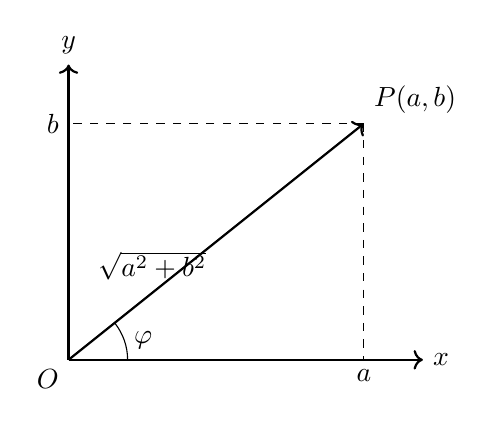
\begin{tikzpicture}[scale=1.5]
    \draw[->, thick] (0,0) -- (3,0) node[right] {$x$};
    \draw[->, thick] (0,0) -- (0,2.5) node[above] {$y$};
    \draw[->, thick] (0,0) -- (2.5, 2) node [above right] {$P(a,b)$};
    \draw (0.5,0) arc (0:38.66:0.5) node[midway, right] {$\varphi$};
    \draw[dashed] (2.5,2) -- (2.5,0) node[below]{$a$};
    \draw[dashed] (2.5,2) -- (0,2) node[left]{$b$};
    \node at (0,0) [below left] {$O$};
    \node at (1.25, 1) [below left] {$\sqrt{a^2+b^2}$};
\end{tikzpicture}
\end{center}

% ---------------------------------------------
\subsection{积化和差与和差化积公式}
% ---------------------------------------------
\begin{theorembox}{积化和差与和差化积公式}
\begin{itemize}
    \item \textbf{积化和差}
    \begin{align*}
        \sin\alpha\cos\beta &= \frac{1}{2}[\sin(\alpha+\beta) + \sin(\alpha-\beta)] \\
        \cos\alpha\sin\beta &= \frac{1}{2}[\sin(\alpha+\beta) - \sin(\alpha-\beta)] \\
        \cos\alpha\cos\beta &= \frac{1}{2}[\cos(\alpha+\beta) + \cos(\alpha-\beta)] \\
        \sin\alpha\sin\beta &= -\frac{1}{2}[\cos(\alpha+\beta) - \cos(\alpha-\beta)]
    \end{align*}
    \item \textbf{和差化积}
    \begin{align*}
        \sin A + \sin B &= 2\sin\frac{A+B}{2}\cos\frac{A-B}{2} \\
        \sin A - \sin B &= 2\cos\frac{A+B}{2}\sin\frac{A-B}{2} \\
        \cos A + \cos B &= 2\cos\frac{A+B}{2}\cos\frac{A-B}{2} \\
        \cos A - \cos B &= -2\sin\frac{A+B}{2}\sin\frac{A-B}{2}
    \end{align*}
\end{itemize}
\end{theorembox}


\newpage
% =============================================
\section{核心解题思想与技巧}
% =============================================

% ---------------------------------------------
\subsection{齐次关系:知一求三}
% ---------------------------------------------
\begin{examplebox}{“齐次”思想的应用}
在三角函数中,$\sin\alpha$ 和 $\cos\alpha$ 的关系类似于代数中的 $a$ 和 $b$。利用 $(a+b)^2$, $(a-b)^2$, $ab$, $a^2+b^2$ 这四个式子中,知二可求二的代数关系。在三角函数中,由于 $\sin^2\alpha + \cos^2\alpha = 1$ 是恒成立的,所以我们实际上是“知一求三”。

\textbf{问题模型}:已知 $\sin\alpha + \cos\alpha = m$,求 $\sin\alpha - \cos\alpha$, $\sin\alpha\cos\alpha$ 的值。

\textbf{解题步骤}:
\begin{enumerate}
    \item \textbf{求 $\sin\alpha\cos\alpha$}:
    将已知式两边平方:
    \[ (\sin\alpha + \cos\alpha)^2 = m^2 \]
    \[ \sin^2\alpha + 2\sin\alpha\cos\alpha + \cos^2\alpha = m^2 \]
    \[ 1 + 2\sin\alpha\cos\alpha = m^2 \implies \sin\alpha\cos\alpha = \frac{m^2-1}{2} \]

    \item \textbf{求 $\sin\alpha - \cos\alpha$}:
    利用平方差关系:
    \[ (\sin\alpha - \cos\alpha)^2 = \sin^2\alpha - 2\sin\alpha\cos\alpha + \cos^2\alpha = 1 - 2\sin\alpha\cos\alpha \]
    将上一步的结果代入:
    \[ (\sin\alpha - \cos\alpha)^2 = 1 - 2\left(\frac{m^2-1}{2}\right) = 1 - (m^2-1) = 2 - m^2 \]
    因此,
    \[ \sin\alpha - \cos\alpha = \pm\sqrt{2-m^2} \]
    (注意:最终结果的正负需要根据角 $\alpha$ 所在的象限来确定。)
\end{enumerate}
\textbf{示例}:已知 $\sin\alpha + \cos\alpha = \frac{1}{5}$,且 $\alpha \in (0, \pi)$,求 $\sin\alpha - \cos\alpha$。
\begin{itemize}
    \item $2\sin\alpha\cos\alpha = \left(\frac{1}{5}\right)^2 - 1 = -\frac{24}{25} \implies \sin\alpha\cos\alpha = -\frac{12}{25} < 0$。
    因为 $\alpha \in (0, \pi)$,$\sin\alpha > 0$,所以 $\cos\alpha < 0$。角 $\alpha$ 在第二象限。
    \item $(\sin\alpha - \cos\alpha)^2 = 2 - (\frac{1}{5})^2 = \frac{49}{25}$。
    \item $\sin\alpha - \cos\alpha = \pm\frac{7}{5}$。
    \item 因为 $\alpha$ 在第二象限,$\sin\alpha > 0$, $\cos\alpha < 0$,所以 $\sin\alpha - \cos\alpha > 0$。
    故 $\sin\alpha - \cos\alpha = \frac{7}{5}$。
\end{itemize}
\end{examplebox}

% ---------------------------------------------
\subsection{弦化切与切化弦}
% ---------------------------------------------
\begin{examplebox}{弦切互化技巧}
\textbf{弦化切}:当一个分式表达式的分子分母都是关于 $\sin\alpha$ 和 $\cos\alpha$ 的一次齐次式时,可以通过分子分母同除以 $\cos\alpha$ 来简化计算。

\textbf{示例}:计算 $\frac{\sin\alpha - 2\cos\alpha}{3\sin\alpha + 4\cos\alpha}$,已知 $\tan\alpha = 3$。
\[ \frac{\sin\alpha - 2\cos\alpha}{3\sin\alpha + 4\cos\alpha} = \frac{\frac{\sin\alpha}{\cos\alpha} - 2\frac{\cos\alpha}{\cos\alpha}}{3\frac{\sin\alpha}{\cos\alpha} + 4\frac{\cos\alpha}{\cos\alpha}} = \frac{\tan\alpha - 2}{3\tan\alpha + 4} = \frac{3-2}{3(3)+4} = \frac{1}{13} \]

\textbf{切化弦}:将式子中的 $\tan\alpha$ 全部换成 $\frac{\sin\alpha}{\cos\alpha}$,然后通分化简。这在证明恒等式时非常常用。
\end{examplebox}

% =============================================
\section{三角形内的三角函数结论}
% =============================================
\begin{theorembox}{三角形内常用结论}
在任意 $\triangle ABC$ 中,有 $A+B+C=\pi$。由此可得:
\begin{itemize}
    \item \textbf{角的关系}:
        \[ A+B = \pi - C \quad \implies \quad \frac{A+B}{2} = \frac{\pi}{2} - \frac{C}{2} \]
    \item \textbf{诱导公式的应用}:
        \begin{align*}
            \sin(A+B) &= \sin(\pi - C) = \sin C \\
            \cos(A+B) &= \cos(\pi - C) = -\cos C \\
            \tan(A+B) &= \tan(\pi - C) = -\tan C \\
            \sin\left(\frac{A+B}{2}\right) &= \sin\left(\frac{\pi}{2} - \frac{C}{2}\right) = \cos\frac{C}{2} \\
            \cos\left(\frac{A+B}{2}\right) &= \cos\left(\frac{\pi}{2} - \frac{C}{2}\right) = \sin\frac{C}{2}
        \end{align*}
    \item \textbf{重要恒等式}:若 $A+B+C=\pi$,则
        \begin{equation}
            \tan A + \tan B + \tan C = \tan A \tan B \tan C
        \end{equation}
        \textbf{推论}:若 $\tan A + \tan B + \tan C > 0$,则 $\triangle ABC$ 为锐角三角形。若 $\tan A \tan B \tan C > 0$,则也为锐角三角形。
\end{itemize}
\end{theorembox}

% =============================================
\section{解三角不等式}
% =============================================
\begin{examplebox}{解不等式 $\sin x > \cos x$}
解这类不等式通常有两种方法:
\begin{enumerate}
    \item \textbf{图像法}:在同一坐标系中画出 $y=\sin x$ 和 $y=\cos x$ 的图像。不等式 $\sin x > \cos x$ 的解集即为 $y=\sin x$ 图像在 $y=\cos x$ 图像上方的部分对应的 $x$ 的取值范围。
    
    \begin{center}
    \begin{tikzpicture}[domain=-pi/2:2*pi, samples=200, scale=1.2]
        \draw[->] (-pi/2-0.2, 0) -- (2*pi+0.2, 0) node[right] {$x$};
        \draw[->] (0,-1.2) -- (0,1.2) node[above] {$y$};
        
        \draw[myblue, thick] plot (\x, {sin(\x r)});
        \draw[myred, dashed, thick] plot (\x, {cos(\x r)});
        
        \fill[myblue!20, domain=pi/4:5*pi/4] plot(\x, {sin(\x r)}) -- (5*pi/4, {cos(5*pi/4 r)}) -- plot[domain=5*pi/4:pi/4] (\x, {cos(\x r)}) -- (pi/4, {sin(pi/4 r)});

        \draw[dotted] (pi/4, -1.2) node[below] {$\frac{\pi}{4}$} -- (pi/4, {sin(pi/4 r)});
        \draw[dotted] (5*pi/4, -1.2) node[below] {$\frac{5\pi}{4}$} -- (5*pi/4, {sin(5*pi/4 r)});
        \node at (pi*1.2, 1) {\color{myblue}\Large $\sin x > \cos x$};
    \end{tikzpicture}
    \end{center}
    从图中可以看出,在一个周期内,解集为 $x \in \left(\frac{\pi}{4}, \frac{5\pi}{4}\right)$。
    所以通解为:$x \in \left(2k\pi + \frac{\pi}{4}, 2k\pi + \frac{5\pi}{4}\right), k \in \mathbb{Z}$。

    \item \textbf{单位圆法}:在单位圆上,$\sin x = y_P$, $\cos x = x_P$。不等式 $\sin x > \cos x$ 转化为 $y_P > x_P$。直线 $y=x$ 与单位圆的交点所对应的角为 $\frac{\pi}{4}$ 和 $\frac{5\pi}{4}$。在单位圆上位于直线 $y=x$ 上方的弧所对应的角的范围即为解集。
    
    \begin{center}
    \begin{tikzpicture}[scale=1.5]
        \draw[->] (-1.5,0) -- (1.5,0) node[right] {$x$};
        \draw[->] (0,-1.5) -- (0,1.5) node[above] {$y$};
        \draw[thin, mygray] (0,0) circle (1);
        \draw[dashed] (-1.2, -1.2) -- (1.2, 1.2) node[right] {$y=x$};
        
        \coordinate (A) at (45:1);
        \coordinate (B) at (225:1);
        
        \draw[myblue, very thick] (A) arc (45:225:1);
        \node[color=myblue, below right] at (A) {$P(\cos x, \sin x)$};
        \node at (-1, 1) {\color{myblue}\Large $y > x$};

        \draw[->, dotted] (0.5,0) arc (0:45:0.5);
        \node at (0.8,0.2) {$\frac{\pi}{4}$};
        \draw[->, dotted, dashed] (0.7,0) arc (0:225:0.7);
        \node at (-0.3, -0.7) {$\frac{5\pi}{4}$};
    \end{tikzpicture}
    \end{center}
    单位圆法同样得到解集为 $x \in \left(2k\pi + \frac{\pi}{4}, 2k\pi + \frac{5\pi}{4}\right), k \in \mathbb{Z}$。
\end{enumerate}
\end{examplebox}


\end{document}
% --- 文档结束 ---
